%!TEX program = xelatex+makeindex+bibtex
\documentclass[final]{scrreprt} %scrreprt of scrartcl
% Include all project wide packages here.
\usepackage{fullpage}
\usepackage{polyglossia}
\setmainlanguage{english}
\usepackage{csquotes}
\usepackage{graphicx}
\usepackage{epstopdf}
\usepackage{pdfpages}
\usepackage{caption}
\usepackage[list=true]{subcaption}
\usepackage{float}
\usepackage{standalone}
\usepackage{import}
\usepackage{tocloft}
\usepackage{wrapfig}
\usepackage{authblk}
\usepackage{array}
\usepackage{booktabs}
\usepackage[toc,page,title,titletoc]{appendix}
\usepackage{xunicode}
\usepackage{fontspec}
\usepackage{pgfplots}
\usepackage{SIunits}
\usepackage{units}
\pgfplotsset{compat=newest}
\pgfplotsset{plot coordinates/math parser=false}
\newlength\figureheight 
\newlength\figurewidth
\usepackage{amsmath}
\usepackage{mathtools}
\usepackage{unicode-math}
\usepackage[
    backend=bibtexu,
	texencoding=utf8,
bibencoding=utf8,
    style=ieee,
    sortlocale=en_US,
    language=auto
]{biblatex}
\usepackage{listings}
\newcommand{\includecode}[3][c]{\lstinputlisting[caption=#2, escapechar=, style=#1]{#3}}
\newcommand{\superscript}[1]{\ensuremath{^{\textrm{#1}}}}
\newcommand{\subscript}[1]{\ensuremath{_{\textrm{#1}}}}


\newcommand{\chapternumber}{\thechapter}
\renewcommand{\appendixname}{Bijlage}
\renewcommand{\appendixtocname}{Bijlagen}
\renewcommand{\appendixpagename}{Bijlagen}

\usepackage[hidelinks]{hyperref} %<--------ALTIJD ALS LAATSTE

\renewcommand{\familydefault}{\sfdefault}

\setmainfont[Ligatures=TeX]{Myriad Pro}
\setmathfont{Asana Math}
\setmonofont{Lucida Console}

\usepackage{titlesec, blindtext, color}
\definecolor{gray75}{gray}{0.75}
\newcommand{\hsp}{\hspace{20pt}}
\titleformat{\chapter}[hang]{\Huge\bfseries}{\chapternumber\hsp\textcolor{gray75}{|}\hsp}{0pt}{\Huge\bfseries}
\renewcommand{\familydefault}{\sfdefault}
\renewcommand{\arraystretch}{1.2}
\setlength\parindent{0pt}

%For code listings
\definecolor{black}{rgb}{0,0,0}
\definecolor{browntags}{rgb}{0.65,0.1,0.1}
\definecolor{bluestrings}{rgb}{0,0,1}
\definecolor{graycomments}{rgb}{0.4,0.4,0.4}
\definecolor{redkeywords}{rgb}{1,0,0}
\definecolor{bluekeywords}{rgb}{0.13,0.13,0.8}
\definecolor{greencomments}{rgb}{0,0.5,0}
\definecolor{redstrings}{rgb}{0.9,0,0}
\definecolor{purpleidentifiers}{rgb}{0.01,0,0.01}


\lstdefinestyle{csharp}{
language=[Sharp]C,
showspaces=false,
showtabs=false,
breaklines=true,
showstringspaces=false,
breakatwhitespace=true,
escapeinside={(*@}{@*)},
columns=fullflexible,
commentstyle=\color{greencomments},
keywordstyle=\color{bluekeywords}\bfseries,
stringstyle=\color{redstrings},
identifierstyle=\color{purpleidentifiers},
basicstyle=\ttfamily\small}

\lstdefinestyle{c}{
language=C,
showspaces=false,
showtabs=false,
breaklines=true,
showstringspaces=false,
breakatwhitespace=true,
escapeinside={(*@}{@*)},
columns=fullflexible,
commentstyle=\color{greencomments},
keywordstyle=\color{bluekeywords}\bfseries,
stringstyle=\color{redstrings},
identifierstyle=\color{purpleidentifiers},
}

\lstdefinestyle{matlab}{
language=Matlab,
showspaces=false,
showtabs=false,
breaklines=true,
showstringspaces=false,
breakatwhitespace=true,
escapeinside={(*@}{@*)},
columns=fullflexible,
commentstyle=\color{greencomments},
keywordstyle=\color{bluekeywords}\bfseries,
stringstyle=\color{redstrings},
identifierstyle=\color{purpleidentifiers}
}

\lstdefinestyle{vhdl}{
language=VHDL,
showspaces=false,
showtabs=false,
breaklines=true,
showstringspaces=false,
breakatwhitespace=true,
escapeinside={(*@}{@*)},
columns=fullflexible,
commentstyle=\color{greencomments},
keywordstyle=\color{bluekeywords}\bfseries,
stringstyle=\color{redstrings},
identifierstyle=\color{purpleidentifiers}
}

\lstdefinestyle{xaml}{
language=XML,
showspaces=false,
showtabs=false,
breaklines=true,
showstringspaces=false,
breakatwhitespace=true,
escapeinside={(*@}{@*)},
columns=fullflexible,
commentstyle=\color{greencomments},
keywordstyle=\color{redkeywords},
stringstyle=\color{bluestrings},
tagstyle=\color{browntags},
morestring=[b]",
  morecomment=[s]{<?}{?>},
  morekeywords={xmlns,version,typex:AsyncRecords,x:Arguments,x:Boolean,x:Byte,x:Char,x:Class,x:ClassAttributes,x:ClassModifier,x:Code,x:ConnectionId,x:Decimal,x:Double,x:FactoryMethod,x:FieldModifier,x:Int16,x:Int32,x:Int64,x:Key,x:Members,x:Name,x:Object,x:Property,x:Shared,x:Single,x:String,x:Subclass,x:SynchronousMode,x:TimeSpan,x:TypeArguments,x:Uid,x:Uri,x:XData,Grid.Column,Grid.ColumnSpan,Click,ClipToBounds,Content,DropDownOpened,FontSize,Foreground,Header,Height,HorizontalAlignment,HorizontalContentAlignment,IsCancel,IsDefault,IsEnabled,IsSelected,Margin,MinHeight,MinWidth,Padding,SnapsToDevicePixels,Target,TextWrapping,Title,VerticalAlignment,VerticalContentAlignment,Width,WindowStartupLocation,Binding,Mode,OneWay,xmlns:x}
}

%defaults
\lstset{
basicstyle=\ttfamily\small,
extendedchars=false,
numbers=left,
numberstyle=\ttfamily\tiny,
stepnumber=1,
tabsize=4,
numbersep=5pt
}
\addbibresource{../../library/bibliography.bib}
\begin{document}

\chapter{System Integration}
\label{ch:system-integration}
We use a program written in C\# and C++ to control the car.
The full source in included in Appendix listing \ref{app:source}.
For a little bit of overview of the source, there is a code map included in Appendix \ref{app:code-map}, this contains all important classes.
Only a couple are omitted.
First, we will quickly explain the different components of the program.
After that we will go into some extra detail on why we choose this approach.
A system diagram is shown in figure \ref{fig:system-diagram}.
For any implementation details please consult the source code.
\begin{figure}[H]
	\centering    	
    	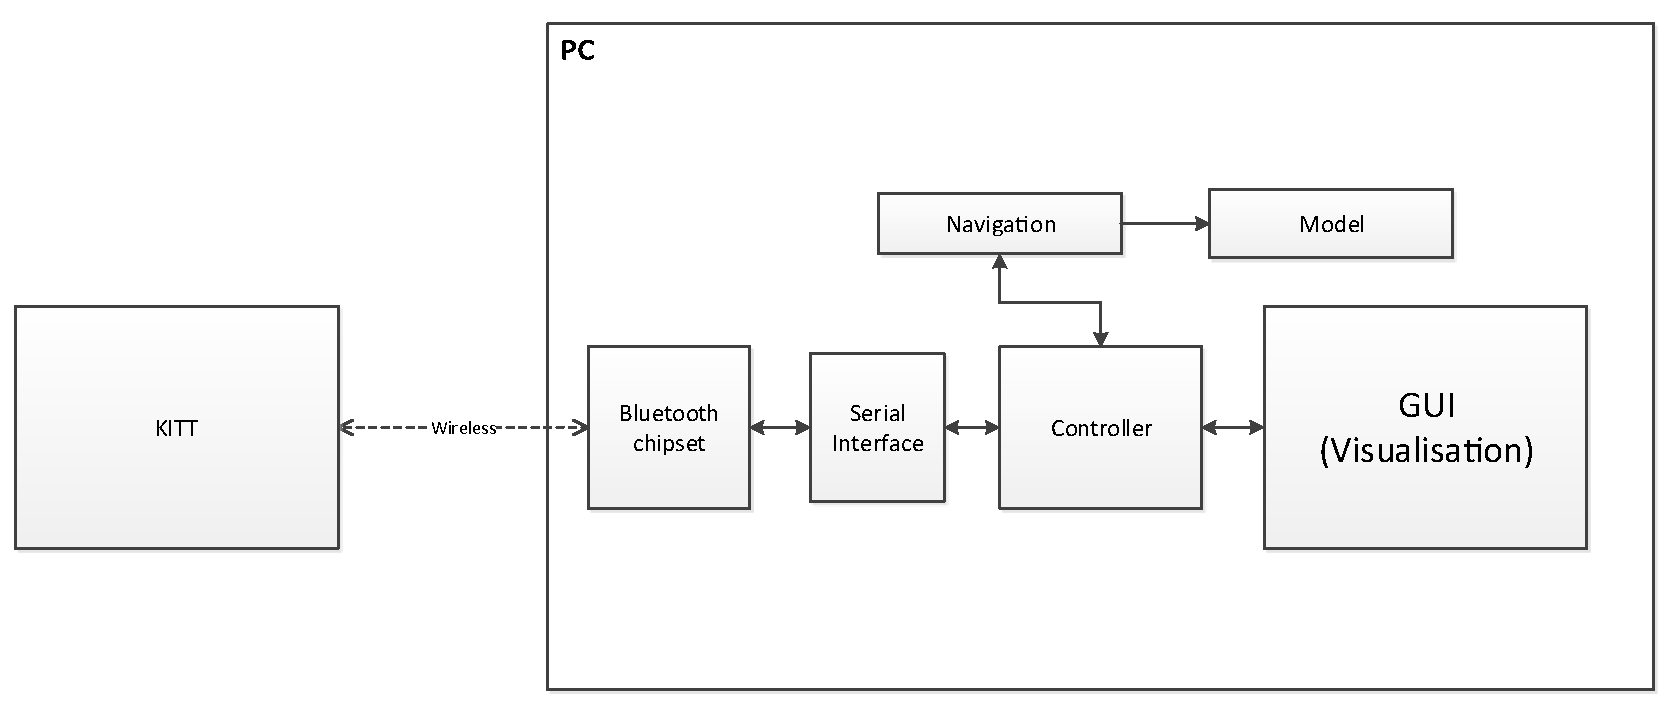
\includegraphics[width=\textwidth]{resources/system-diagram.pdf}
    	\caption{The system in diagram form}
    	\label{fig:system-diagram}
\end{figure}
\section{Modules}
This is a short list of the current components.
\begin{itemize}
\item Visualization
\item Controller
\item Navigation
\item Model
\item Communication
\item ASIO
\end{itemize}
\section{Controller}
ASIO is the interface with the 8 channel capture card.
The controller is the part that gives the car it's behavior.
The Controller is parent to the Navigation and thus the Model.
The navigation class is the class with the role of observer and the Model class in the class with the role of controller (in a state-space sense).
We use a kind of double state-space model (the state is now a 2 by 2 matrix), this gives us two ``driving'' signals one for the x and one for the y direction.
From these two we can take the actual driving signal (the magnitude of the vector) and the steering signal (the difference with the current bearing).
We use a deadzone of \SI{0.2}{\radian}, so when the absolute value if the bearing difference is smaller then that the car won't steer.
The steering signal is to the left is the bearing difference is bigger than the deadzone and is to the right when the bearing difference is smaller then the deadzone.\\
A problem arises when you want to estimate the bearing for previous measured position and the car is moving very slowly. 
When the positions are very close to each other, the error might be bigger than the actual distance traveled.
This makes the bearing determined completely wrong.
The first thing we did to tackle this problem was, we made the car go faster and the position measurement rate lower (from \SI{4}{\hertz} to \SI{2}{\hertz}).
This helped a lot, the car now drives in a nice smooth arc to it's destination, it's a shame the steering signals were flipped in the demo.\\
After all these small things, which could have been easily fixed with a bit more testing time, the car drives in a quite direct manner to it's destination.
The controller does have an automatic emergency stop (anti-collision), when an object gets to close it brakes the car immediately.
We take the previously measured position and set this as the target, the result is that the car nearly stops on the spot.
This was also used, in a simpler form, in the wall driving test.


\section{System response}
In figure \ref{fig:system-response} you can see the data of a run towards the wall.
\begin{figure}[H]
	\centering
    	\setlength\figureheight{4cm}
    	\setlength\figurewidth{0.8\linewidth}
    	% This file was created by matlab2tikz v0.4.6 running on MATLAB 8.3.
% Copyright (c) 2008--2014, Nico Schlömer <nico.schloemer@gmail.com>
% All rights reserved.
% Minimal pgfplots version: 1.3
% 
% The latest updates can be retrieved from
%   http://www.mathworks.com/matlabcentral/fileexchange/22022-matlab2tikz
% where you can also make suggestions and rate matlab2tikz.
% 
\begin{tikzpicture}

\begin{axis}[%
width=\figurewidth,
height=\figureheight,
scale only axis,
xmin=0,
xmax=4.5,
xlabel={t (s)},
ymin=-20,
ymax=310,
ylabel={x (cm) \& input signal},
legend style={draw=black,fill=white,legend cell align=left}
]
\addplot [color=blue,solid]
  table[row sep=crcr]{
0	300	\\
0.1	300	\\
0.2	300	\\
0.3	300	\\
0.4	300	\\
0.5	300	\\
0.6	301	\\
0.7	288	\\
0.8	288	\\
0.9	274	\\
1	259	\\
1.1	243	\\
1.2	225	\\
1.3	206	\\
1.4	184	\\
1.5	184	\\
1.6	164	\\
1.7	143	\\
1.8	120	\\
1.9	96	\\
2	71	\\
2.1	71	\\
2.2	46	\\
2.3	26	\\
2.4	16	\\
2.5	14	\\
2.6	14	\\
2.7	13	\\
2.8	13	\\
2.9	13	\\
3	13	\\
3.1	13	\\
3.2	13	\\
3.3	14	\\
3.4	14	\\
3.5	14	\\
3.6	15	\\
3.7	15	\\
3.8	14	\\
3.9	14	\\
4	15	\\
4.1	15	\\
4.2	15	\\
4.3	16	\\
4.4	16	\\
4.5	15	\\
};
\addlegendentry{Sensordata Right};

\addplot [color=black!50!green,solid]
  table[row sep=crcr]{
0	300	\\
0.1	301	\\
0.2	301	\\
0.3	300	\\
0.4	300	\\
0.5	300	\\
0.6	304	\\
0.7	292	\\
0.8	292	\\
0.9	279	\\
1	265	\\
1.1	249	\\
1.2	230	\\
1.3	213	\\
1.4	191	\\
1.5	191	\\
1.6	171	\\
1.7	149	\\
1.8	127	\\
1.9	104	\\
2	78	\\
2.1	78	\\
2.2	54	\\
2.3	30	\\
2.4	16	\\
2.5	11	\\
2.6	12	\\
2.7	10	\\
2.8	10	\\
2.9	10	\\
3	10	\\
3.1	10	\\
3.2	10	\\
3.3	11	\\
3.4	11	\\
3.5	11	\\
3.6	12	\\
3.7	12	\\
3.8	12	\\
3.9	11	\\
4	12	\\
4.1	12	\\
4.2	12	\\
4.3	13	\\
4.4	13	\\
4.5	12	\\
};
\addlegendentry{Sensordata Left};

\addplot [color=red,solid]
  table[row sep=crcr]{
0	8	\\
0.1	8	\\
0.2	8	\\
0.3	8	\\
0.4	8	\\
0.5	8	\\
0.6	8	\\
0.7	8	\\
0.8	8	\\
0.9	8	\\
1	8	\\
1.1	8	\\
1.2	8	\\
1.3	8	\\
1.4	8	\\
1.5	8	\\
1.6	8	\\
1.7	0	\\
1.8	6	\\
1.9	-8	\\
2	-10	\\
2.1	-14	\\
2.2	8	\\
2.3	-15	\\
2.4	-15	\\
2.5	0	\\
2.6	0	\\
2.7	0	\\
2.8	-9	\\
2.9	0	\\
3	0	\\
3.1	-8	\\
3.2	0	\\
3.3	0	\\
3.4	0	\\
3.5	-7	\\
3.6	0	\\
3.7	0	\\
3.8	-7	\\
3.9	0	\\
4	0	\\
4.1	0	\\
4.2	-7	\\
4.3	0	\\
4.4	0	\\
4.5	-7	\\
};
\addlegendentry{Input signals};

\end{axis}

\begin{axis}[%
width=\figurewidth,
height=\figureheight,
scale only axis,
xmin=0,
xmax=1,
ymin=0,
ymax=1,
hide axis,
axis x line*=bottom,
axis y line*=left
]
\addplot [color=black,solid,line width=0.0pt,mark=square*,mark options={solid,fill=black,draw=white},forget plot]
  table[row sep=crcr]{
0.5	0.989690721649485	\\
};
\addplot [color=black,solid,line width=0.0pt,mark=square*,mark options={solid,fill=black,draw=white},forget plot]
  table[row sep=crcr]{
0.992175273865415	0.5	\\
};
\addplot [color=black,solid,line width=0.0pt,mark=square*,mark options={solid,fill=black,draw=white},forget plot]
  table[row sep=crcr]{
0.5	0.0103092783505155	\\
};
\addplot [color=black,solid,line width=0.0pt,mark=square*,mark options={solid,fill=black,draw=white},forget plot]
  table[row sep=crcr]{
0.00782472613458529	0.5	\\
};
\addplot [color=black,solid,line width=0.0pt,mark=square*,mark options={solid,fill=black,draw=white},forget plot]
  table[row sep=crcr]{
0.00782472613458529	0.989690721649485	\\
};
\addplot [color=black,solid,line width=0.0pt,mark=square*,mark options={solid,fill=black,draw=white},forget plot]
  table[row sep=crcr]{
0.992175273865415	0.0103092783505155	\\
};
\addplot [color=black,solid,line width=0.0pt,mark=square*,mark options={solid,fill=black,draw=white},forget plot]
  table[row sep=crcr]{
0.992175273865415	0.989690721649485	\\
};
\addplot [color=black,solid,line width=0.0pt,mark=square*,mark options={solid,fill=black,draw=white},forget plot]
  table[row sep=crcr]{
0.00782472613458529	0.0103092783505155	\\
};
\end{axis}
\end{tikzpicture}%    	
    	\caption{The system response of the “drive-to-wall command”.}
    	\label{fig:system-response}
\end{figure}

\section{Implementation details and Licenses}
All our code and documentation with be available on GitHub, shortly after the project at \href{https://github.com/EraYaN}{https://github.com/EraYaN}. The repositories' name is \href{https://github.com/EraYaN/EV2020}{EV2020}. All our own code is released under the Creative Commons Attribution-NonCommercial-ShareAlike 4.0 International, available at \href{http://creativecommons.org/licenses/by-nc-sa/4.0/}{CreativeCommons}.
Third-party code retain their respective licenses.\\

We used the following libraries/SDKs.
\begin{itemize}
\item ASIOSDK 2.3
\item BlueWave.Interop.Asio
\item CircularBuffer
\item MicroMvvm
\item MathNet.Numerics master@83f222f02
\item Intel MKL 11.1 update 3
\item OxyPlot.Core 2014.1.240.1
\item OxyPlot.Wpf 2014.1.240.1
\end{itemize}
All their dependencies and licenses are listed on the projects' websites.
\\ \\
\begin{figure}[h]
	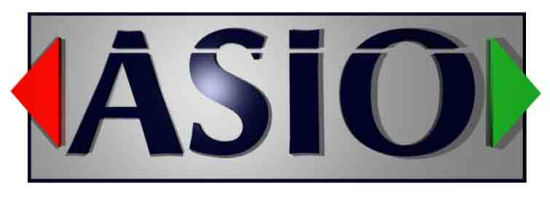
\includegraphics[width=2cm]{resources/ASIO_LOGO1.jpg}
\end{figure}
ASIO Driver Interface Technology by Steinberg Media Technologies GmbH.\\
\begin{figure}[h]
	
\includegraphics[width=2cm]{resources/intel-logo.jpg}
\end{figure}
Intel Math Kernel Library by Intel Corporation.

\end{document}